\setlength{\parskip}{1em}

\begin{tikzpicture}
  \node (Professor) [anchor=north west, inner sep=0pt] at (current page.north) {\input{./tex/Professor_v5.tex}};
  \node[right = 0.1 of Professor, yshift=0cm, xshift=0cm] (Multimuons1) {\begin{multimuons-1}[enhanced, tikz={rotate=0}]{CDF publishes multi-muons!}
  \begin{multicols}{2}
    We report a study of multi-muon events produced at the
    Fermilab Tevatron collider and recorded by the CDF~II detector. In a data 
    set acquired with a dedicated dimuon trigger and corresponding to an 
    integrated luminosity of 2100 pb$^{-1}$, we isolate a significant sample of 
    events in which at least one of the muon candidates is produced 
    outside of the beam pipe of radius 1.5 cm. The production cross section
    and kinematics of events in which both muon candidates are produced inside
    the beam pipe are successfully modeled by known QCD processes which
    include heavy flavor production. In contrast, we are presently unable to 
    fully account for the number and properties of the remaining events, in which
    at least one muon candidate is produced outside of the beam pipe, in terms
    of the same understanding of the CDF~II detector, trigger, and event 
    reconstruction. Several topological and kinematic properties of these 
    events are presented in this paper. These events offer a plausible 
    resolution to long-standing inconsistencies related to $b\bar{b}$
    production and decay.
    \begin{comment}
    % ========================
    \begin{figure}
      \begin{center}
        \vspace{-0.2in}
        \leavevmode
        \includegraphics[width=\textwidth]{./figures/MultiMuons1BW_CDF.png}
        %\caption[] {Impact parameter distribution of muons contributed by ghost
        %  ($\bullet$) and QCD (histogram) events. Muon tracks are
        %  selected with loose SVX requirements. The detector resolution
        %  is $\simeq 30 \; \mu$m, whereas bins are 80 $\mu$m wide.} 
      \end{center}
    \end{figure}
    % ========================
    \end{comment}
  \end{multicols}
\end{multimuons-1}
};
  \node[left = 0.1 of Professor] (Fermilab) {\input{./tex/FermilabToday_v2.tex}};
  \node[below = 0.1 of Professor] (IPPOG) {% Ημερίδα πρακτικής άσκησης με δεδομένα από το CERN - Σάββατο 7 Μάρτη 9:00 - 17:00
\begin{MyArticle}[enhanced, tikz={rotate=0}, width=0.3\textwidth]{Master of Masterclasses}
  \begin{multicols}{2}
    Another particle physics masterclass was organized at the University of Cyprus
    by Professor Fotios Ptochos for the 8$^{th}$ year
    in a row. It took within the framework of the IPPOG effort,  with
    the aim of informing young students about the research being
    carried out at CERN and the wider field of Particle Physics.
    Department of Physics. The event you took place on Saturday 07 March
    2020 at the University of Cyprus Campus between 9:00 - 17:00. It 
    included lectures about the world of elementary particles,
    detection methods, and the technology developed starting with
    basic research in both this and related fields of physics. Students had a unique opportunity to
    analyze data from proton-proton collisions, as recorded by the CMS
    detector at CERN's LHC. They discussed their
    findings with students from other countries as well as scientists
    at CERN through a video conference.
    % ========================
    \begin{figure}
      \begin{center}
        \leavevmode
        %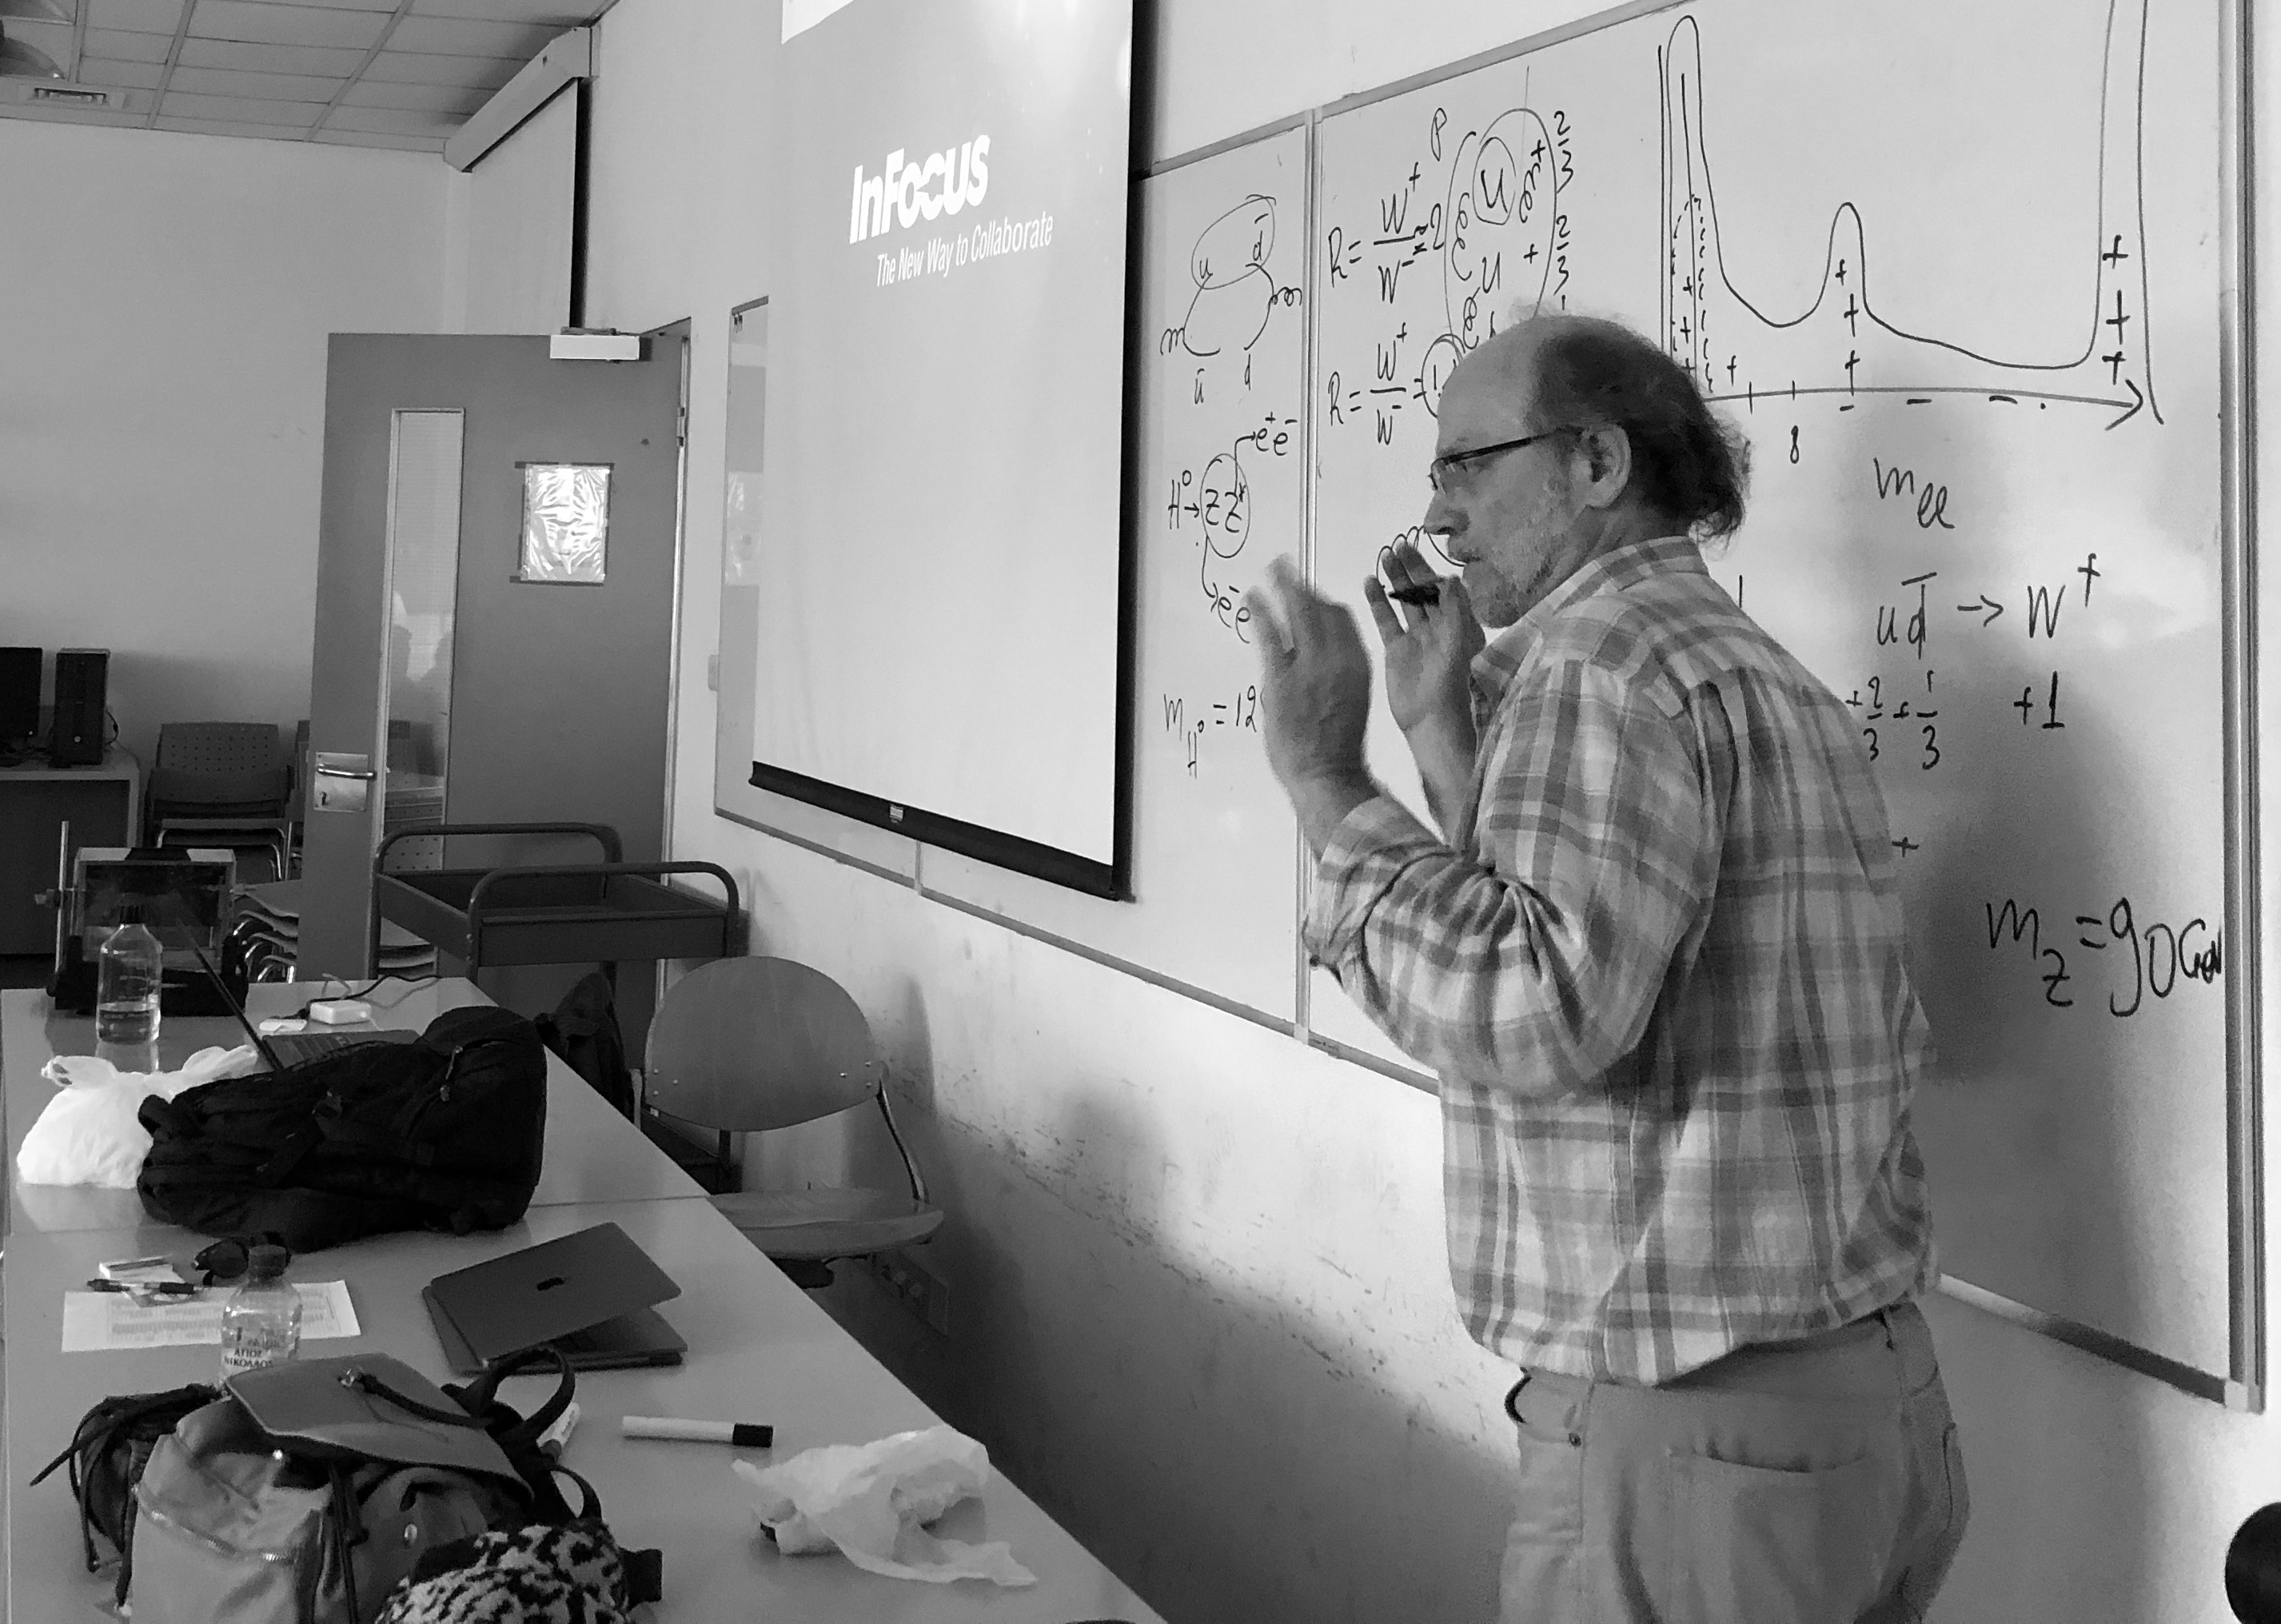
\includegraphics[width=0.45\textwidth]{./figures/Fotis6.png}
        %\includegraphics[width=0.5\textwidth]{./figures/Fotis6-narrow.png}
        %\includegraphics[width=0.4\textwidth]{./figures/Fotis6-small.png}
        \includegraphics[width=0.4\textwidth]{./figures/Fotis6-narrow.png}
      \end{center}
    \end{figure}
    % ========================
  \end{multicols}
\end{MyArticle}
};
  \node[left = 0.1 of IPPOG] (Higgs) {%\begin{MyArticle}[enhanced, height=0.2\textheight,
%tikz={rotate=0}]{Physicists Find Elusive Particle Seen as Key to
%Universe}
\begin{MyArticle}[enhanced, tikz={rotate=0}, width=0.33\textwidth]{Physicists Find Elusive Particle Seen as Key to Universe}
  \begin{multicols}{2}
    Results are presented from searches for the standard model Higgs
    boson in proton–proton collisions at and 8 TeV in the Compact Muon
    Solenoid experiment at the LHC, using data samples corresponding
    to integrated luminosities of up to 5.1 fb$^{−1}$ at 7 TeV and 5.3 fb$^{−1}$
    at 8 TeV. The search is performed in five decay modes:
    $\gamma\gamma$, $ZZ$,  $\tau^{+}\tau^{-}$, and $b\bar{b}$.
    An excess of events is observed above the expected background,
    with a local significance of 5.0 standard deviations, at a mass
    near 125 GeV, signalling the production of a new particle. The
    expected significance for a standard model Higgs boson of that
    mass is 5.8 standard deviations. The excess is most significant in
    the two decay modes with the best mass resolution, $\gamma\gamma$ and $ZZ$; a
    fit to these signals gives a mass of 
    $125.3\pm0.4(\text{stat.})\pm0.5(\text{syst.}$ GeV. The decay to
    two photons indicates that the new particle is a boson with spin 
    different from one. 
    % ========================
    \begin{figure}
      \begin{center}
        \vspace{-0.2in}
        \leavevmode
        \includegraphics[width=0.5\textwidth]{./figures/HiggsBosonDiscoveryBW.png}
      \end{center}
    \end{figure}
    % ========================
  \end{multicols}
\end{MyArticle}
};
  \node[right = 0.1 of IPPOG] (Top) {% new tcolorbox environment
\newtcolorbox{topQuark}[2][]{
  coltext      = black,
  colframe     = \MyBlockFrameColorLeft,
  colback      = \MyBlockFillColorLeft,
  colbacktitle = \MyBlockTitleBoxColor,
  coltitle     = black,
  title        = {\Large{\textbf{#2}}},
  fonttitle    = \bfseries,
  boxrule      = 0.2cm, %frame line width
  %tikz={rotate=#3}, % manipulate the tcolorbox as a whole (in degrees)
  top=+0.0cm, bottom=+0.0cm, left=+0.05cm, right=+0.05cm,
  %enlarge top by   = +1.0cm,  %  equivalent to mdframed 'skipabove'
  %enlarge bottom by= +0.0cm,  %  equivalent to mdframed 'skipbelow'
  %enlarge left by  = +1.5cm,  
  %enlarge right by = +0.0cm, 
  opacityback=1.0, % 1.0 means totally transparent, 0.0 means totally opaque
  arc=0.0cm,        % 0.0cm for non-rounded corners!
  #1,
}


\begin{topQuark}[enhanced, tikz={rotate=0}]{Top Quark, Last Piece of Matter, Appears to Be in Place}
  \begin{multicols}{2}
    We establish the existence of the top quark using a 67 pb$^{-1}$ data
    sample of pp collisions at $\sqrt{s} = 1.8$ TeV collected with the Collider
    Detector at Fermilab (CDF). Employing techniques similar to those we
    previously published, we observe a signal consistent with $t\bar{t}$ decay to
    $WWbb$, but inconsistent with the background prediction by
    4.8$\sigma$. Additional evidence for the top quark is provided by a peak in
    the reconstructed mass distribution. We measure the top quark mass
    to be $176 \pm 8 (\text{stat.}) \pm 10 (\text{sys.})$ GeV/c$^{2}$,
    and the $t\bar{t}$ production cross section to be
    $6.8^{+3.6}_{-2.4}$ pb.
    % ========================
    \begin{figure}
      \begin{center}
        \vspace{-0.2in}
        \leavevmode
        \includegraphics[width=0.5\textwidth]{./figures/TopQuarkAnnouncement.jpg}
      \end{center}
    \end{figure}
    % ========================
  \end{multicols}
\end{topQuark}
};
  \node[below = 0.1 of Higgs] (CMS-HIG-18-015) {\begin{MyArticleDotted}[enhanced, tikz={rotate=0}, width=0.25\textwidth]{Search for charged Higgs bosons!} %
  \begin{multicols}{2}
    A search for charged Higgs bosons ($H^{\pm}$) decaying into a top
    and a bottom quark in the all-jet final state is presented. The
    analysis uses LHC proton-proton collision data recorded with the
    CMS detector in 2016 at $\sqrt{s} = 13$ TeV, corresponding to an
    integrated luminosity of 35.9~$fb^{-1}$. No significant excess is
    observed above the expected background. Model-independent upper
    limits at 95$\%$ confidence level are set on the product of the
    $H^{\pm}$ production cross section and branching fraction in two
    scenarios.  For production in association with a top quark,
    limits of 21.3 to 0.007$pb$ are obtained for $H^{\pm}$ masses in the
    range of 0.2 to 3 TeV. Combining this with a search in leptonic
    final states results in improved limits of 9.25 to 0.005 $pb$. The
    complementary $s$-channel production of an $H^{\pm}$ is
    investigated in the mass range of 0.8 to 3 TeV and the
    corresponding upper limits are 4.5 to 0.023 $pb$. These results are
    interpreted using different minimal supersymmetric extensions of
    the standard model.
 \end{multicols}
\end{MyArticleDotted}
};  
  \node[right = 0.1 of CMS-HIG-18-015] (Multimuons2) {% new tcolorbox environment
\newtcolorbox{topQuark}[2][]{
  coltext      = black,
  colframe     = \MyBlockFrameColorLeft,
  colback      = \MyBlockFillColorLeft,
  colbacktitle = \MyBlockTitleBoxColor,
  coltitle     = black,
  title        = {\Large{\textbf{#2}}},
  fonttitle    = \bfseries,
  boxrule      = 0.2cm, %frame line width
  %tikz={rotate=#3}, % manipulate the tcolorbox as a whole (in degrees)
  top=+0.0cm, bottom=+0.0cm, left=+0.05cm, right=+0.05cm,
  %enlarge top by   = +1.0cm,  %  equivalent to mdframed 'skipabove'
  %enlarge bottom by= +0.0cm,  %  equivalent to mdframed 'skipbelow'
  %enlarge left by  = +1.5cm,  
  %enlarge right by = +0.0cm, 
  opacityback=1.0, % 1.0 means totally transparent, 0.0 means totally opaque
  arc=0.0cm,        % 0.0cm for non-rounded corners!
  #1,
}

% CMS
\begin{topQuark}[enhanced, tikz={rotate=0}]{Multi-Muons In CDF: The Mystery Continues}
  %\begin{multicols}{2}
    We present a phenomenological conjecture of new physics that is suggested
    by the topology and kinematic properties of the multi-muon events recently
    reported by the CDF collaboration. We show that the salient features of 
    the data can be accounted for by postulating the pair production of
    three new states $h_1$, $h_2$, and $h_3$ with masses in the range
    of 15, 7.3, and 3.6 GeV/c$^{2}$, respectively. The heavier states 
    cascade-decay into the lighter ones, whereas the lightest state 
    decays into a $\tau$ pair with a lifetime of the order of 20 ps.
    \begin{comment}
    % ========================
    \begin{figure}
      \begin{center}
        \vspace{-0.2in}
        \leavevmode
        \includegraphics[width=\textwidth]{./figures/MultiMuons2_CDF.pdf}
        %\caption[]{Two-dimensional distributions, reproduced from Ref.~\cite{a0disc},
        %  of (a) the invariant mass, $M$, of all muons and (b) the total
        %  number of tracks contained in a $36.8^{\deg}$ cone when both
        %  cones contain at least two muons.}
      \end{center}
    \end{figure}
    % ========================
    \end{comment}
%  \end{multicols}
\end{topQuark}
};
  \node[right = 0.1 of Multimuons2] (CMS-HIG-21-010) {% Higgs boson: a tool to discover new physics: $H^{\pm}$
\begin{MyArticle}[enhanced, tikz={rotate=0}, boxrule=1pt, titlerule=0pt, width=0.25\textwidth]{New
    search for charged Higgs bosons in forgotten channels}
  \begin{multicols}{2}
  A search for a charged Higgs boson $H^{\pm}$ decaying
  into a heavy neutral Higgs boson $H$ and a $W$ boson
  is presented. The analysis targets the $W$ decay into a pair
  of tau leptons with at least one of them decaying hadronically and
  with an additional electron or muon present in the event.
  The search is based on proton-proton collision data
  recorded by the CMS experiment during 2016--2018 at
  $\sqrt{s} = 13~TeV$, corresponding to an integrated
  luminosity of 138~$fb^{-1}$. The data are consistent with
  standard model background expectations. Upper limits at 95$\%$ confidence
  level are set on the product of the cross section and branching fraction
  for an $H^{\pm}$ in the mass range of 300--700 GeV, assuming an $H$ 
  with a mass of 200 GeV. The observed limits range from
  0.085 $pb$ for an $H^{\pm}$ mass of
  300 $GeV$ to 0.019~$pb$ for a mass of
  700 $GeV$. These are the first limits on $H^{\pm}$
  production in the $H^{\pm} \to H W^{\pm}$ decay channel at the LHC. 
  \end{multicols}
\end{MyArticle}
};
 \node[left = 0.1 of CMS-HIG-21-010] (NASA) {%F.Ptochos hosting ``NASA Missions: From the Sun to Pluto and Beyond'' speech at University of Cyprus by Dr. James L. Green.
\begin{MyArticle}[enhanced, tikz={rotate=0}, width=0.25\textwidth]{From the Sun to Pluto and Beyond}
  On \longdate\formatdate{19}{10}{2018} a public lecture was given by Dr. James L. Green, NASA Chief Scientist, at
  the University House \say{Anastasios G. Leventis} of the University
  of Cyprus. The speaker was introduced by Associate Professor Fotios
  Ptochos, Chairperson of the Department of Physics. The event was
  organized by the University of Cyprus in cooperation with the
  U.S. Embassy Cyprus and Cyprus Space Exploration Organisation (CSEO).
  \begin{figure}
      \begin{center}
        \leavevmode
        %\includegraphics[width=0.4\textwidth]{./figures/NASA.jpg}
        \includegraphics[width=0.8\textwidth]{./figures/NASA-small.png}
      \end{center}
    \end{figure}
    % ========================
\end{MyArticle}
};
  %  \node[left = 0.2cm of IPPOG] (HExtented) {\begin{MyArticle}[enhanced, tikz={rotate=0}]{Charged Higgs boson
    Hunting}
  $t\rightarrow bH^{\pm}\rightarrow \tau^{\pm} \nu_{\tau}$............................\it{25 May 2012}\newline
  $H^{\pm}\rightarrow tb$ and $H^{\pm}\rightarrow \tau\nu$..............\it{31 August 2015}\newline
  $H^{\pm} \rightarrow \tau^{\pm} \nu_{\tau}$ ................................\it{11 March 2019}\newline
  $pp\rightarrow t(b)H^{\pm} \rightarrow tb$, all-jet.......\it{21 January 2020}\newline
  $pp\rightarrow t(b)H^{\pm} \rightarrow W^{\pm}H^{0}(\tau\tau)$...............\it{4 July 2022}
  %\begin{tabular}{l l}
%  \hline
%  \bf $H^{\pm} \rightarrow \tau^{\pm} \nu_{\tau}$  & \it{11 March 2019}\\
%  \bf $H^{\pm} \rightarrow tb$, all-jet            & \it{21 January 2020}\\
%  \bf $H^{\pm} \rightarrow W^{\pm}H^{0}(\tau\tau)$ & \it{4 July 2022}\\
%  \hline
%\end{tabular}
\end{MyArticle}
% https://cms-results.web.cern.ch/cms-results/public-results/publications/HIG-11-019/index.html
% https://cms-results.web.cern.ch/cms-results/public-results/publications/HIG-14-023/index.html
% https://cms-results.web.cern.ch/cms-results/public-results/publications/HIG-18-014/index.html
% https://cms-results.web.cern.ch/cms-results/public-results/publications/HIG-18-015/index.html
% https://cms-results.web.cern.ch/cms-results/public-results/publications/HIG-21-010/index.html
};
 %\node[below = 0.1 of Multimuons1] (Ads1) {\begin{MyAd}[enhanced, tikz={rotate=0},  width=0.25\textwidth]{}% 
  Visit your favorite spots in town for amazing dishes and wine!
  \begin{figure}
    \begin{center}
      \vspace{-0.5cm}
      \includegraphics[width=1.0\textwidth]{./figures/restaurants.png}
    \end{center}
  \end{figure}
  \vspace{-0.5cm}
\end{MyAd}
};
 \node[below = 0.1 of Multimuons1] (Ads1) {\begin{MyAd}[enhanced, tikz={rotate=0},  width=0.25\textwidth]{}% 
  Visit your favorite spots in town for amazing dishes and wine!
  \begin{figure}
    \begin{center}
      \vspace{-0.5cm}
      \includegraphics[width=1.0\textwidth]{./figures/restaurants.png}
    \end{center}
  \end{figure}
  \vspace{-0.5cm}
\end{MyAd}
};
\end{tikzpicture}
